%%%%%%%%%%%%%%%%%%%%%%%%%%%%%%%%%%%%%%%%%
% Fancyslides Presentation
% LaTeX Template
% Version 1.0 (30/6/13)
%
% This template has been downloaded from:
% http://www.LaTeXTemplates.com
%
% The Fancyslides class was created by:
% Paweł Łupkowski (pawel.lupkowski@gmail.com)
%
% License:
% CC BY-NC-SA 3.0 (http://creativecommons.org/licenses/by-nc-sa/3.0/)
%
%%%%%%%%%%%%%%%%%%%%%%%%%%%%%%%%%%%%%%%%%

%----------------------------------------------------------------------------------------
%	PACKAGES AND OTHER DOCUMENT CONFIGURATIONS
%----------------------------------------------------------------------------------------

\documentclass{fancyslides}

\usepackage[utf8]{inputenc} % Allows the usage of non-english characters
\usepackage{times} % Use the Times font
\usepackage{booktabs} % Allows the use of \toprule, \midrule and \bottomrule in tables
\graphicspath{{images/}} % Location of the slide background and figure files

% Beamer options - do not change
\usetheme{default} 
\setbeamertemplate{navigation symbols}{} % Disable the slide navigation buttons on the bottom of each slide
\setbeamercolor{structure}{fg=\yourowntexcol} % Define the color of titles and fixed text elements (e.g. bullet points)
\setbeamercolor{normal text}{fg=\yourowntexcol} % Define the color of text in the presentation

%------------------------------------------------
% COLORS
% The following colors are predefined in this class: white, black, gray, blue, green and orange

% Define your own color as follows:
%\definecolor{pink}{rgb}{156,0,151}

\newcommand{\structureopacity}{0.75} % Opacity (transparency) for the structure elements (boxes and circles)

\newcommand{\strcolor}{blue} % Set the color of structure elements (boxes and circles)
\newcommand{\yourowntexcol}{white} % Set the text color

%----------------------------------------------------------------------------------------
%	TITLE SLIDE
%----------------------------------------------------------------------------------------

\newcommand{\titlephrase}{GDA SCORE \\
\LARGE General Data Anonymity Score} % Presentation title
\newcommand{\name}{Ramy Chemak} % Presenter's name
\newcommand{\affil}{Computer science laboratory of Orléans} % Presenter's institution
\newcommand{\email}{INSA Centre Val de Loire} % Presenter's email address
\begin{document}

\startingslide % This command inserts the title slide as the first slide

%----------------------------------------------------------------------------------------
%	PRESENTATION SLIDES
%----------------------------------------------------------------------------------------

%------------------------------------------------

\fbckg{blank} % Slide background image
\begin{frame}
\pointedsl{Introduction}
\end{frame}

%------------------------------------------------

%\fbckg{gda_score_logo.jpeg} % Slide background image
\begin{frame}
\misc{ % Anything can be placed inside the \misc{} command
\Huge
\begin{enumerate}
\centering
\item \textcolor{current_s}{Data Privacy}
\item Anonymization models
\end{enumerate}
}
\end{frame}

%------------------------------------------------

%\fbckg{2.jpg} % Slide background image
\begin{frame}
\itemized{ % This environment simply prints a series of bullet points
\item Mass personal data mining
\item Threats for data privacy
\item Scandals over personal data leaks
}
\end{frame}

%------------------------------------------------

%\fbckg{gda_score_logo.jpeg} % Slide background image
\begin{frame}
\misc{ % Anything can be placed inside the \misc{} command
\begin{quote}
"Anonymisation results from processing personal data in order to irreversibly prevent identification [\ldots]"
\end{quote}
\begin{flushright}
\textbf{Article 29 Data Protection Working Party Opinion 05/2014 on Anonymisation Tecniques}
\end{flushright}
}
\end{frame}

%------------------------------------------------

\iffalse
%\fbckg{gda_score_logo.jpeg} % Slide background image
\begin{frame}
\misc{ % Anything can be placed inside the \misc{} command
\begin{quote}
"the principles of protection must apply to any information concerning an identified or identifiable person; whereas, to determine whether a person is identifiable, account should be taken of all the means likely reasonably to be used either by the controller or by any other person to identify the said person [\ldots]"
\end{quote}
\begin{flushright}
\textbf{Article 29 Data Protection Working Party Opinion 05/2014 on Anonymisation Tecniques}
\end{flushright}
}
\end{frame}
\fi

%------------------------------------------------

%\fbckg{gda_score_logo.jpeg} % Slide background image
\begin{frame}
\misc{ % Anything can be placed inside the \misc{} command
\Huge
\begin{enumerate}
\centering
\item Data Privacy
\item \textcolor{current_s}{Anonymization models}
\end{enumerate}
}
\end{frame}

%------------------------------------------------

%\fbckg{2.jpg} % Slide background image
\begin{frame}
\itemized{ % This environment simply prints a series of bullet points
\item Pseudonymization \\ \newline \newline
\begin{quote} \small \newline
"the processing of personal data in such a manner that the personal data can no longer be attributed to a specific data subject without the use of additional information \ldots"
\end{quote}
\begin{flushright}
\textbf{ \small GDPR - Article 4}
\end{flushright}
}
\end{frame}

%------------------------------------------------

%\fbckg{2.jpg} % Slide background image
\begin{frame}
\itemized{ % This environment simply prints a series of bullet points
\item \textcolor{red}{Pseudonymization}
\item K-Anonymity \newline \newline \small
A dataset is considered k-anonymous if each record is indistinguishable from at least k-1 other records regarding a particular QID. Each obtained cluster defines an equivalent class.
%\newline \Rightarrow defines an equivalent class
}
\end{frame}

%------------------------------------------------

%\fbckg{2.jpg} % Slide background image
\begin{frame}
\itemized{ % This environment simply prints a series of bullet points
\item \textcolor{red}{Pseudonymization}
\item K-Anonymity
\item L-Diversity \newline \newline \small
An equivalence class is considered l-diverse if, for some sensitive attribute, we have l distinct values.
}
\end{frame}

%------------------------------------------------

\begin{frame}
\begin{center}
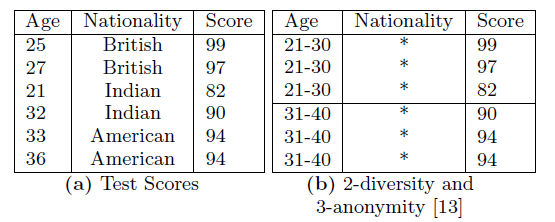
\includegraphics[width=1\linewidth]{sem04.png}
\end{center}
\begin{flushright}
\\ \\ \small
\textcolor{grey}{\textbf{Source:} V. Rastogi, D. Suciu, S. Hong. The Boundary between Privacy and Utility in data publishing, 2007.}
\end{flushright}
\end{frame}

%------------------------------------------------

%\fbckg{2.jpg} % Slide background image
\begin{frame}
\itemized{ % This environment simply prints a series of bullet points
\item \textcolor{red}{Pseudonymization}
\item K-Anonymity
\item L-Diversity
\item Differential privacy \newline \newline \small
Differential privacy provides a guarantee that information about a specific individual cannot be leaked or
disclosed just regarding its membership.
}
\end{frame}

%------------------------------------------------

\begin{frame}
\begin{center}
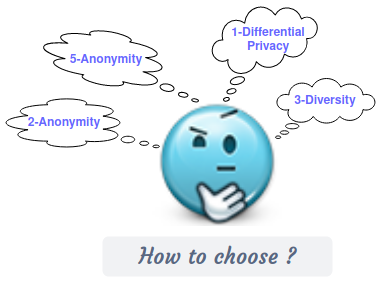
\includegraphics[width=1\linewidth]{anon.png}
\end{center}
\end{frame}

%------------------------------------------------

%\fbckg{1.jpg} % Slide background image
\begin{frame}
\pointedsl{GDA Score}
\end{frame}

%------------------------------------------------

%\fbckg{gda_score_logo.jpeg} % Slide background image
\begin{frame}
\misc{ % Anything can be placed inside the \misc{} command
\Huge
\begin{enumerate}
\centering
\item \textcolor{current_s}{Presentation}
\item Defense \& Utility metrics
\item GDA Score API
\item Feedback
\end{enumerate}
}
\end{frame}

%------------------------------------------------

%\fbckg{2.jpg} % Slide background image
\begin{frame}
%\misc{ % Anything can be placed inside the \misc{} command
%Schema for the four classes
\begin{center}

\includegraphics[width=1\linewidth]{gda_score_logo.jpeg}

\includegraphics[width=1\linewidth]{mpi-sws.jpeg}
\end{center}
%}
\end{frame}

%------------------------------------------------

%\fbckg{2.jpg} % Slide background image
\begin{frame}
\itemized{ % This environment simply prints a series of bullet points
\item Software + API
\item Compares defense and utility measurements
}
\end{frame}

%------------------------------------------------

%\fbckg{gda_score_logo.jpeg} % Slide background image
\begin{frame}
\misc{ % Anything can be placed inside the \misc{} command
\Huge
\begin{enumerate}
\centering
\item Presentation
\item \textcolor{current_s}{Defense \& Utility metrics}
\item GDA Score API
\item Feedback
\end{enumerate}
}
\end{frame}

%------------------------------------------------

%\fbckg{2.jpg} % Slide background image
\begin{frame}
\misc{
\LARGE Attack process
\begin{center}
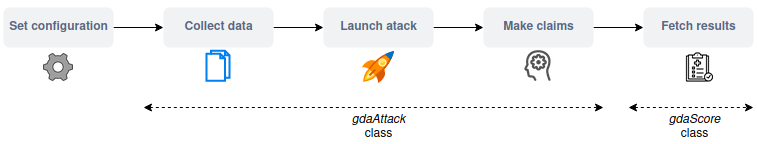
\includegraphics[width=1\linewidth, height=2.7cm]{workflow.png}
\newline \large \textcolor{black}{Attack's algorithm workflow}
\end{center}
}
\end{frame}

%------------------------------------------------

%\fbckg{2.jpg} % Slide background image
\begin{frame}
\misc{
\LARGE Defense metrics
\itemized{ % This environment simply prints a series of bullet points
\item Depends on 3 criteria
}
}
\end{frame}

%------------------------------------------------

%\fbckg{2.jpg} % Slide background image
\begin{frame}
\misc{
\LARGE Defense metrics
\itemized{ % This environment simply prints a series of bullet points
\item Depends on 3 criteria \\
\tab 1. Singling out
}
}
\end{frame}

%------------------------------------------------

%\fbckg{2.jpg} % Slide background image
\begin{frame}
\misc{
\LARGE Defense metrics
\itemized{ % This environment simply prints a series of bullet points
\item Depends on 3 criteria \\
\tab 1. Singling out \\
\tab 2. Inference
}
}
\end{frame}

%------------------------------------------------

%\fbckg{2.jpg} % Slide background image
\begin{frame}
\misc{
\LARGE Defense metrics
\itemized{ % This environment simply prints a series of bullet points
\item Depends on 3 criteria \\
\tab 1. Singling out \\
\tab 2. Inference \\
\tab 3. Linkability
}
}
\end{frame}

%------------------------------------------------

\begin{frame}
\begin{center}
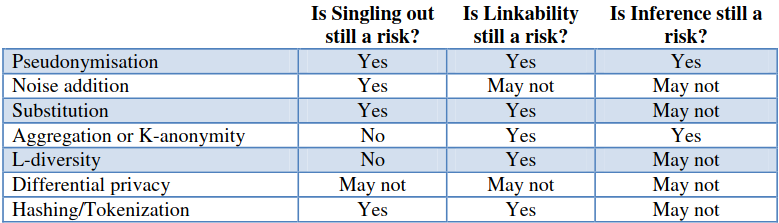
\includegraphics[width=1\linewidth]{wp29.png}
\end{center}
\begin{flushright}
\\ \\ \small
\textcolor{grey}{\textbf{Source:} Article 29 Data Protection Working Party Opinion 05/2014 on Anonymisation Tecniques.}
\end{flushright}
\end{frame}

%------------------------------------------------

%\fbckg{2.jpg} % Slide background image
\begin{frame}
\misc{
\LARGE Defense metrics
\itemized{ % This environment simply prints a series of bullet points
\item Depends on 3 criteria
\item Based on 5 scores
}
}
\end{frame}

%------------------------------------------------

%\fbckg{2.jpg} % Slide background image
\begin{frame}
\misc{
\LARGE Defense metrics
\itemized{ % This environment simply prints a series of bullet points
\item Depends on 3 criteria
\item Based on 5 scores \\ \normalsize
- \criteria{Susceptibility:} amount of attackable data
}
}
\end{frame}

%------------------------------------------------

%\fbckg{2.jpg} % Slide background image
\begin{frame}
\misc{
\LARGE Defense metrics
\itemized{ % This environment simply prints a series of bullet points
\item Depends on 3 criteria
\item Based on 5 scores \\ \normalsize
- \criteria{Susceptibility:} amount of attackable data \\
- \criteria{Prior knowledge:} amount of already known information
}
}
\end{frame}

%------------------------------------------------

%\fbckg{2.jpg} % Slide background image
\begin{frame}
\misc{
\LARGE Defense metrics
\itemized{ % This environment simply prints a series of bullet points
\item Depends on 3 criteria
\item Based on 5 scores \\ \normalsize
- \criteria{Susceptibility:} amount of attackable data \\
- \criteria{Prior knowledge:} amount of already known information \\
- \criteria{Confidence improvement:} attacked data considering attackable data
}
}
\end{frame}

%------------------------------------------------

%\fbckg{2.jpg} % Slide background image
\begin{frame}
\misc{
\LARGE Defense metrics
\itemized{ % This environment simply prints a series of bullet points
\item Depends on 3 criteria
\item Based on 5 scores \\ \normalsize
- \criteria{Susceptibility:} amount of attackable data \\
- \criteria{Prior knowledge:} amount of already known information \\
- \criteria{Confidence improvement:} attacked data considering attackable data\\
- \criteria{Claim probability:} accuracy of made claims
}
}
\end{frame}

%------------------------------------------------

%\fbckg{2.jpg} % Slide background image
\begin{frame}
\misc{
\LARGE Defense metrics
\itemized{ % This environment simply prints a series of bullet points
\item Depends on 3 criteria
\item Based on 5 scores \\ \normalsize
- \criteria{Susceptibility:} amount of attackable data \\
- \criteria{Prior knowledge:} amount of already known information \\
- \criteria{Confidence improvement:} attacked data considering attackable data\\
- \criteria{Claim probability:} accuracy of made claims \\
- \criteria{Work:} number of required queries for the attack
}
}
\end{frame}

%------------------------------------------------

%\fbckg{2.jpg} % Slide background image 
\begin{frame}
%\misc{ % Anything can be placed inside the \misc{} command
%Schema for the four classes
\begin{center}
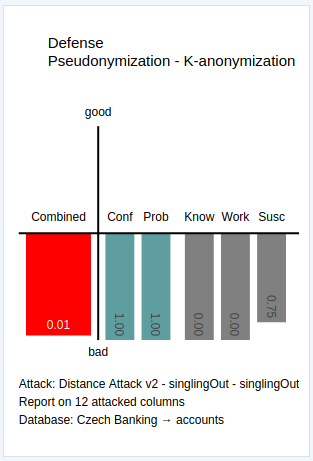
\includegraphics[width=0.5\linewidth]{sem05.png} \\
\textcolor{black}{Defense metrics}
\end{center}
%}
\end{frame}

%------------------------------------------------

%\fbckg{2.jpg} % Slide background image
\begin{frame}
%\misc{ % Anything can be placed inside the \misc{} command
%Schema for the four classes
\begin{center}
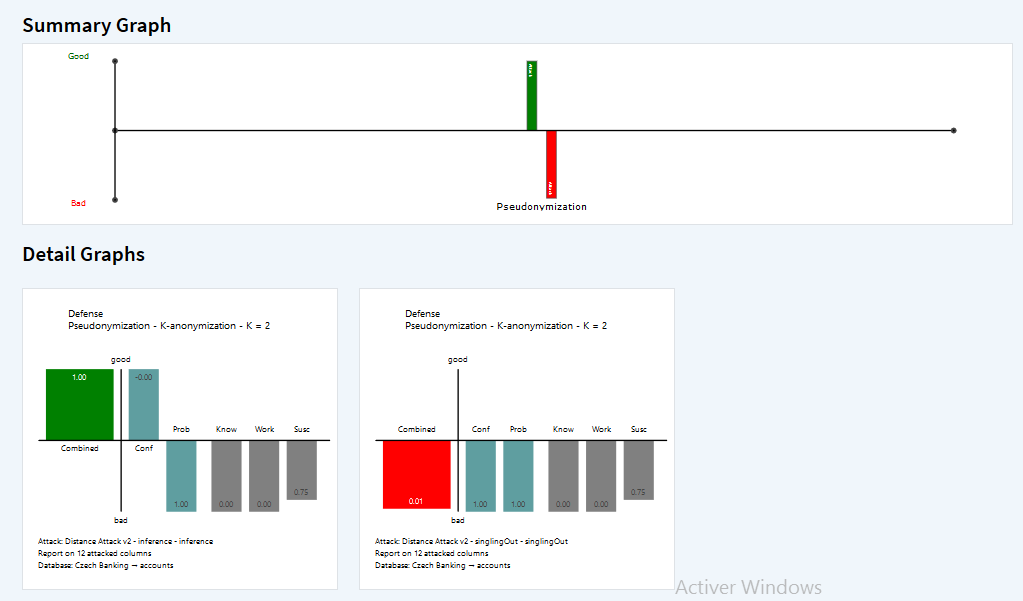
\includegraphics[width=1\linewidth]{sem01.png}
\textcolor{black}{Defense metrics}
\end{center}
%}
\end{frame}

%------------------------------------------------

%\fbckg{2.jpg} % Slide background image
\begin{frame}
\misc{
\LARGE Utility metrics
\itemized{ % This environment simply prints a series of bullet points
\item Based on 2 scores
}
}
\end{frame}

%------------------------------------------------

%\fbckg{2.jpg} % Slide background image
\begin{frame}
\misc{
\LARGE Utility metrics
\itemized{ % This environment simply prints a series of bullet points
\item Based on 2 scores \\
- \criteria{Coverage:} measures lost data
}
}
\end{frame}

%------------------------------------------------

%\fbckg{2.jpg} % Slide background image
\begin{frame}
\misc{
\LARGE Utility metrics
\itemized{ % This environment simply prints a series of bullet points
\item Based on 2 scores \\
- \criteria{Coverage:} measures lost data\\
- \criteria{Accuracy:} measures altered data
}
}
\end{frame}

%------------------------------------------------

%\fbckg{2.jpg} % Slide background image
\begin{frame}
%\misc{ % Anything can be placed inside the \misc{} command
%Schema for the four classes
\begin{center}
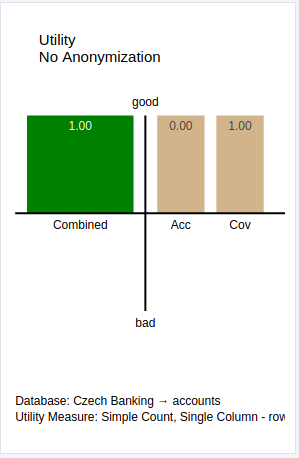
\includegraphics[width=0.5\linewidth]{sem06.png} \\
\textcolor{black}{Utility metrics}
\end{center}
%}
\end{frame}

%------------------------------------------------

%\fbckg{2.jpg} % Slide background image
\begin{frame}
%\misc{ % Anything can be placed inside the \misc{} command
%Schema for the four classes
\begin{center}
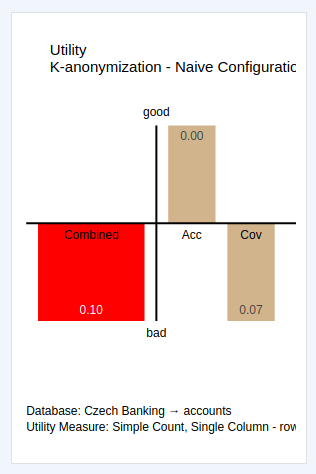
\includegraphics[width=0.5\linewidth]{util02.png} \\
\textcolor{black}{Utility metrics}
\end{center}
%}
\end{frame}

%------------------------------------------------

%\fbckg{2.jpg} % Slide background image
\begin{frame}
%\misc{ % Anything can be placed inside the \misc{} command
%Schema for the four classes
\begin{center}
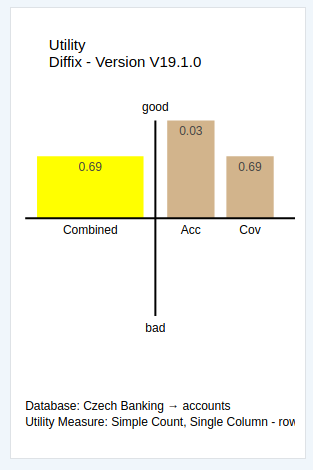
\includegraphics[width=0.5\linewidth]{util03.png} \\
\textcolor{black}{Utility metrics}
\end{center}
%}
\end{frame}

%------------------------------------------------

%\fbckg{gda_score_logo.jpeg} % Slide background image
\begin{frame}
\misc{ % Anything can be placed inside the \misc{} command
\Huge
\begin{enumerate}
\centering
\item Presentation
\item Defense \& Utility metrics
\item \textcolor{current_s}{GDA Score API}
\item Feedback
\end{enumerate}
}
\end{frame}

%------------------------------------------------

%\fbckg{2.jpg} % Slide background image
\begin{frame}
\itemized{ % This environment simply prints a series of bullet points
\begin{flushleft}
\item - Mainly aims at attack scenarios execution
\end{flushleft}
}
\end{frame}

%------------------------------------------------

%\fbckg{2.jpg} % Slide background image
\begin{frame}
%\misc{ % Anything can be placed inside the \misc{} command
%Schema for the four classes
\begin{center}
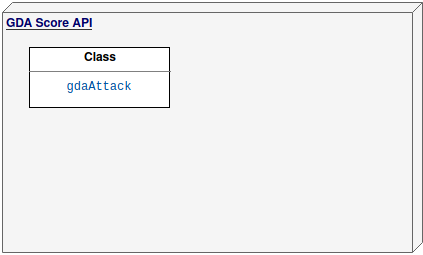
\includegraphics[width=1\linewidth]{api01.png}
\end{center}
%}
\end{frame}

%------------------------------------------------

%\fbckg{2.jpg} % Slide background image
\begin{frame}
%\misc{ % Anything can be placed inside the \misc{} command
%Schema for the four classes
\begin{center}
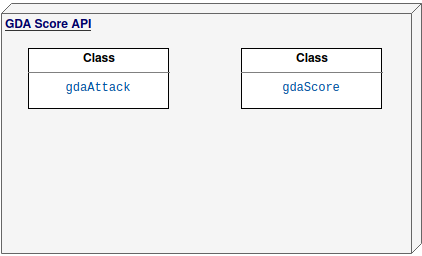
\includegraphics[width=1\linewidth]{api02.png}
\end{center}
%}
\end{frame}

%------------------------------------------------

%\fbckg{2.jpg} % Slide background image
\begin{frame}
%\misc{ % Anything can be placed inside the \misc{} command
%Schema for the four classes
\begin{center}
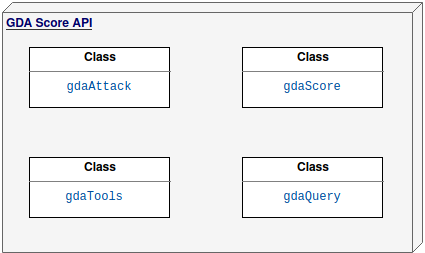
\includegraphics[width=1\linewidth]{api.png}
\end{center}
%}
\end{frame}

%------------------------------------------------

%\fbckg{2.jpg} % Slide background image
\begin{frame}
\itemized{ % This environment simply prints a series of bullet points
\begin{flushleft}
\item - Mainly aims at attacks development
\item - Depends on a GDA distant server
\end{flushleft}
}
\end{frame}

%------------------------------------------------

%\fbckg{2.jpg} % Slide background image
\begin{frame}
\begin{center}
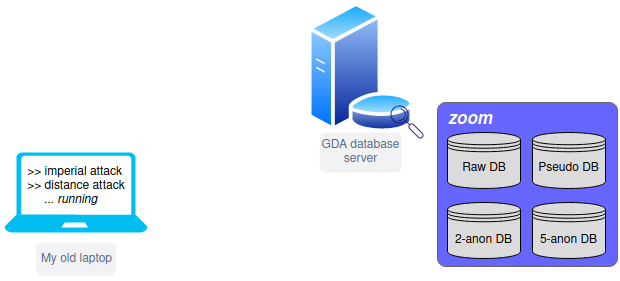
\includegraphics[width=11cm, height=4cm]{attack03.png}
\textcolor{black}{Attack scenario}
\end{center}
\end{frame}

%------------------------------------------------

%\fbckg{2.jpg} % Slide background image
\begin{frame}
\begin{center}
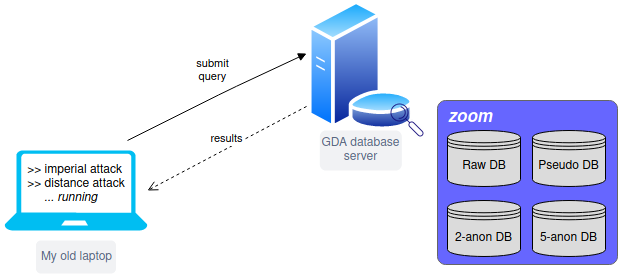
\includegraphics[width=11cm, height=4cm]{attack2.png}
\textcolor{black}{Attack scenario - Static model}
\end{center}
\end{frame}

%------------------------------------------------

%\fbckg{2.jpg} % Slide background image
\begin{frame}
\begin{center}
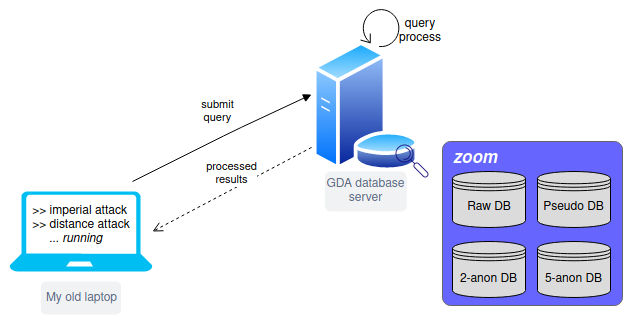
\includegraphics[width=11cm, height=4.5cm]{attack_dynamic.png}
\textcolor{black}{Attack scenario - Dynamic model}
\end{center}
\end{frame}

%------------------------------------------------

%\fbckg{2.jpg} % Slide background image
\begin{frame}
\itemized{ % This environment simply prints a series of bullet points
\begin{flushleft}
\item - Mainly aims at attacks development
\item - Depends on a GDA distant server
\item - Requires a specified attack workflow
\end{flushleft}
}
\end{frame}

%------------------------------------------------

%\fbckg{2.jpg} % Slide background image
\begin{frame}
%\misc{ % Anything can be placed inside the \misc{} command
%Schema for the four classes
\begin{center}
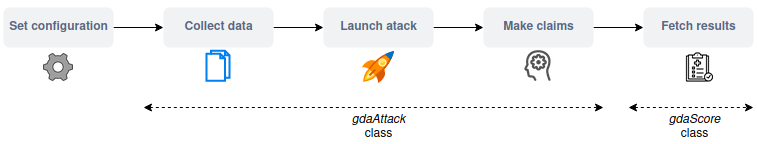
\includegraphics[width=1\linewidth, height=2.7cm]{workflow.png}
\newline \textcolor{black}{Attack's algorithm workflow}
\end{center}
%}
\end{frame}

%------------------------------------------------

%\fbckg{2.jpg} % Slide background image
\begin{frame}
\misc{ % Anything can be placed inside the \misc{} command
\begin{flushleft}
\# Configuration (\texttt{gdaAttack} class)
\newline
\end{flushleft}
}
\end{frame}

%------------------------------------------------

%\fbckg{2.jpg} % Slide background image
\begin{frame}
\misc{ % Anything can be placed inside the \misc{} command
\begin{center}
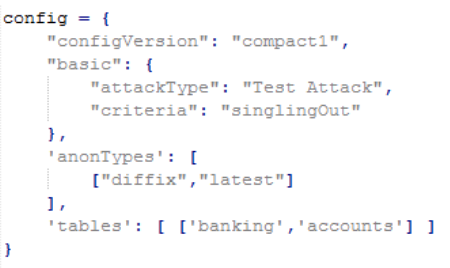
\includegraphics[width=0.8\linewidth]{conf.png}
\textcolor{black}{Configuration}
\end{center}
}
\end{frame}

%------------------------------------------------

%\fbckg{2.jpg} % Slide background image
\begin{frame}
\misc{ % Anything can be placed inside the \misc{} command
\begin{flushleft}
\# Configuration (\texttt{gdaAttack} class)
\newline
\# Prepare the attack (\texttt{askExplore()} \& \texttt{getExplore()})
\newline
\end{flushleft}
}
\end{frame}

%------------------------------------------------

%\fbckg{2.jpg} % Slide background image
\begin{frame}
\misc{ % Anything can be placed inside the \misc{} command
\begin{flushleft}
\# Configuration (\texttt{gdaAttack} class)
\newline
\# Prepare the attack (\texttt{askExplore()} \& \texttt{getExplore()})
\newline
\# Executing the attack (\texttt{askAttack()} \& \texttt{getAttack()})
\newline
\end{flushleft}
}
\end{frame}

%------------------------------------------------

%\fbckg{2.jpg} % Slide background image
\begin{frame}
\misc{ % Anything can be placed inside the \misc{} command
\begin{flushleft}
\# Configuration (\texttt{gdaAttack} class)
\newline
\# Prepare the attack (\texttt{askExplore()} \& \texttt{getExplore()})
\newline
\# Executing the attack (\texttt{askAttack()} \& \texttt{getAttack()})
\newline
\# Making claims (\texttt{True} or \texttt{False})
\newline
\end{flushleft}
}
\end{frame}

%------------------------------------------------

%\fbckg{2.jpg} % Slide background image
\begin{frame}
\misc{ % Anything can be placed inside the \misc{} command
\begin{flushleft}
\# Configuration (\texttt{gdaAttack} class)
\newline
\# Prepare the attack (\texttt{askExplore()} \& \texttt{getExplore()})
\newline
\# Executing the attack (\texttt{askAttack()} \& \texttt{getAttack()})
\newline
\# Making claims (\texttt{True} or \texttt{False})
\newline
\# Grabbing results (\texttt{gdaScore} class)
\newline
\end{flushleft}
}
\end{frame}

%------------------------------------------------

%\fbckg{gda_score_logo.jpeg} % Slide background image
\begin{frame}
\misc{ % Anything can be placed inside the \misc{} command
\Huge
\begin{enumerate}
\centering
\item Presentation
\item Defense \& Utility metrics
\item GDA Score API
\item \textcolor{current_s}{Feedback}
\end{enumerate}
}
\end{frame}

%------------------------------------------------

%\fbckg{2.jpg} % Slide background image
\begin{frame}
\itemized{ % This environment simply prints a series of bullet points
\item Diffix noise-exploitation attack \medskip \\

\includegraphics[width=0.4\linewidth]{imperial_logo.png}

\includegraphics[width=0.4\linewidth]{logo-cpg.png}
}

\end{frame}

%------------------------------------------------

%\fbckg{2.jpg} % Slide background image
\begin{frame}
\itemized{ % This environment simply prints a series of bullet points
\begin{flushleft}
\item - Diffix noise-exploitation attack
\item - Distance-based attack
\end{flushleft}
}
\end{frame}

%------------------------------------------------

%\fbckg{2.jpg} % Slide background image
\begin{frame}
%\misc{ % Anything can be placed inside the \misc{} command
%Schema for the four classes
\begin{center}
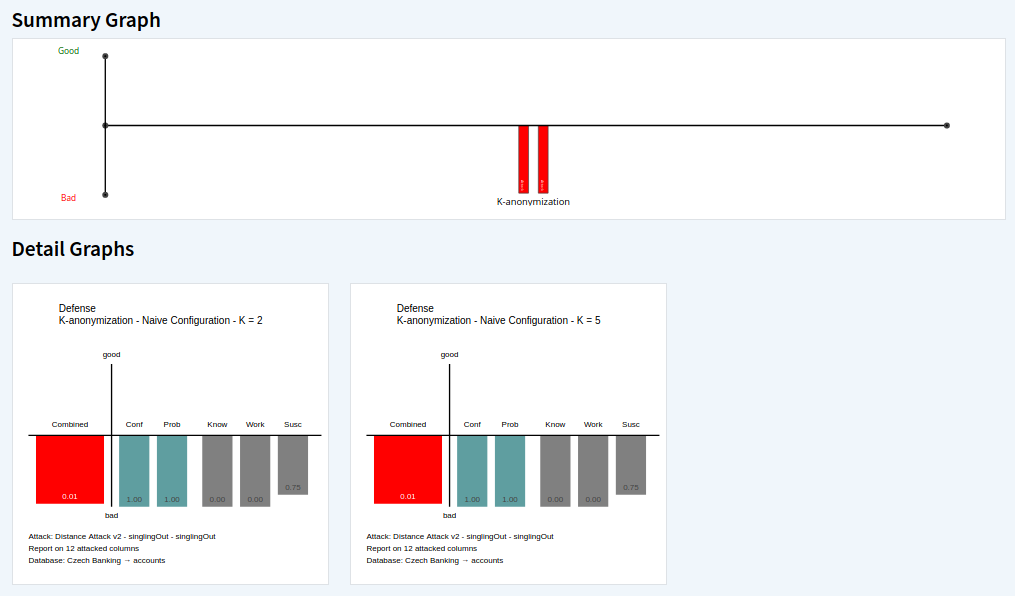
\includegraphics[width=1\linewidth]{distance_results.png}
\textcolor{black}{Results sample}
\end{center}
%}
\end{frame}

%------------------------------------------------

%\fbckg{2.jpg} % Slide background image
\begin{frame}
\itemized{ % This environment simply prints a series of bullet points
\begin{flushleft}
\item - Diffix noise-exploitation attack
\item - Distance-based attack
\item - Software's development progress
\end{flushleft}
}
\end{frame}

%------------------------------------------------

%\fbckg{1.jpg} % Slide background image
\begin{frame}
\pointedsl{Illustration}
\end{frame}

%------------------------------------------------

\fbckg{illust01.png} % Slide background image
\begin{frame}
%\misc{ % Anything can be placed inside the \misc{} command
%Schema for the four classes
%\begin{center}
%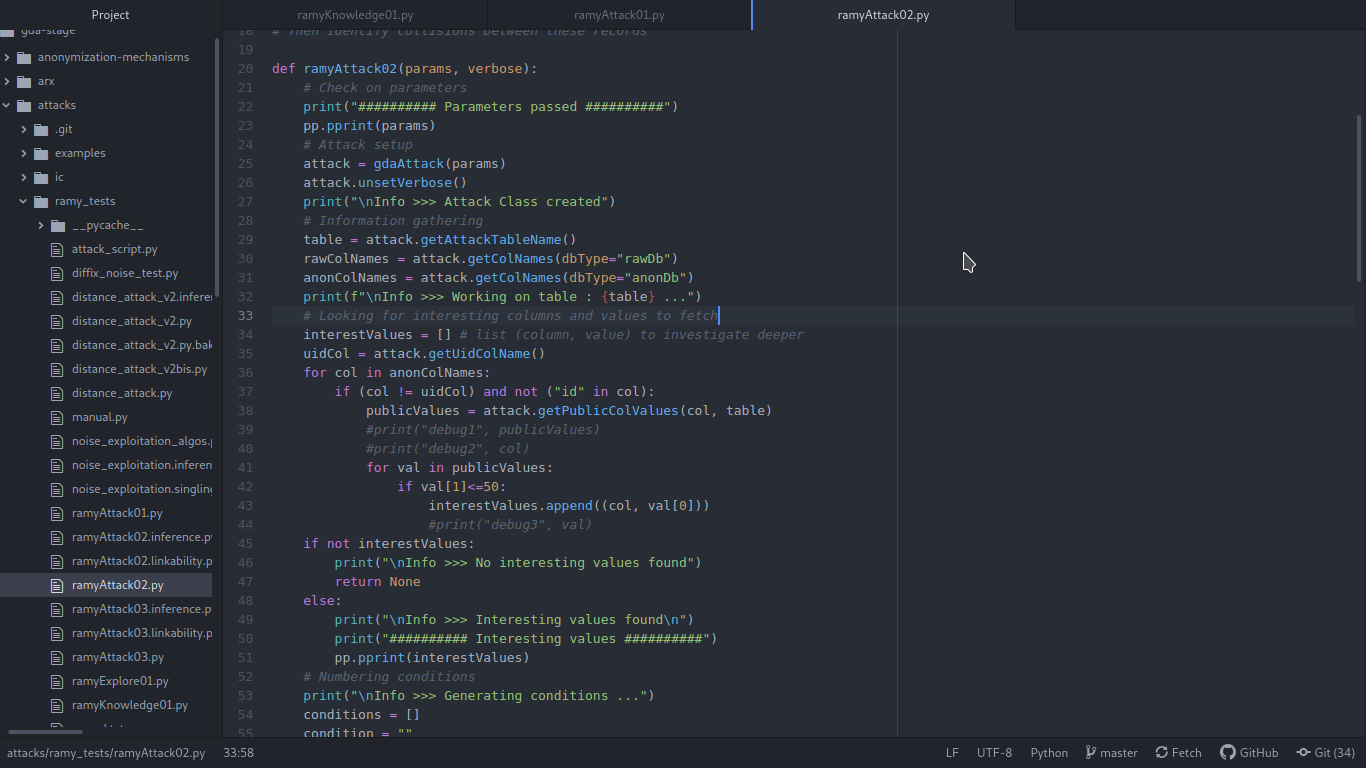
\includegraphics[width=1\linewidth]{illust01.png}
%\end{center}
%}
\end{frame}

%------------------------------------------------

\fbckg{illust02.png} % Slide background image
\begin{frame}
%\misc{ % Anything can be placed inside the \misc{} command
%Schema for the four classes
%\begin{center}
%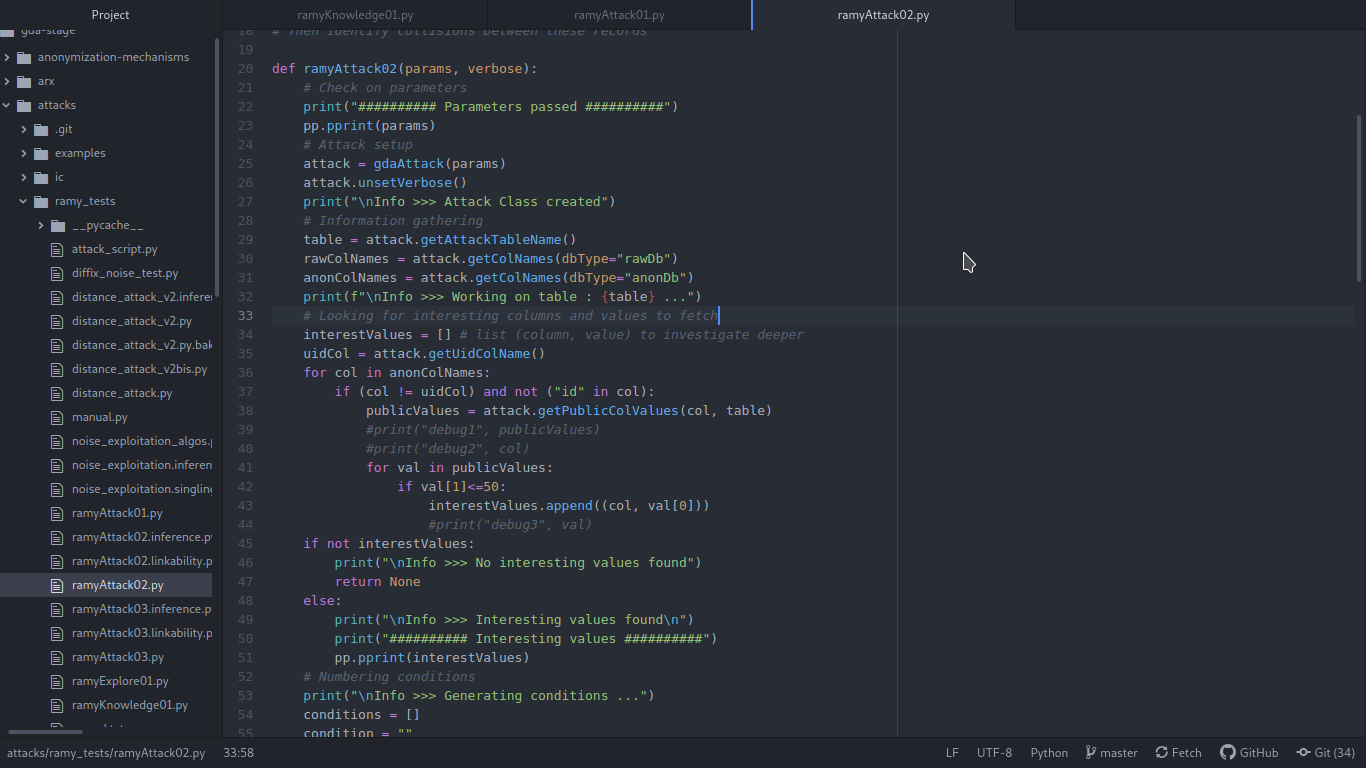
\includegraphics[width=1\linewidth]{illust01.png}
%\end{center}
%}
\end{frame}
%------------------------------------------------

\fbckg{illust03.png} % Slide background image
\begin{frame}
%\misc{ % Anything can be placed inside the \misc{} command
%Schema for the four classes
%\begin{center}
%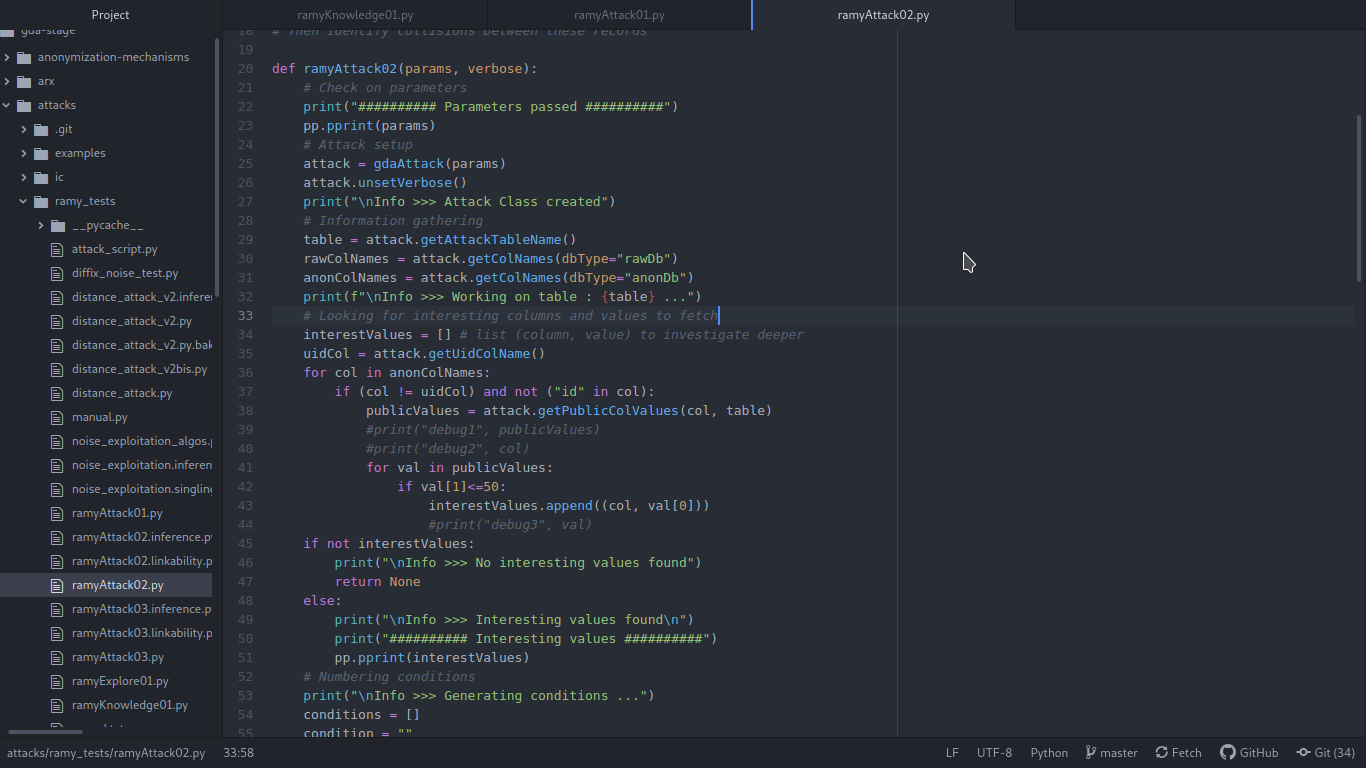
\includegraphics[width=1\linewidth]{illust01.png}
%\end{center}
%}
\end{frame}
%------------------------------------------------

\fbckg{illust04.png} % Slide background image
\begin{frame}
%\misc{ % Anything can be placed inside the \misc{} command
%Schema for the four classes
%\begin{center}
%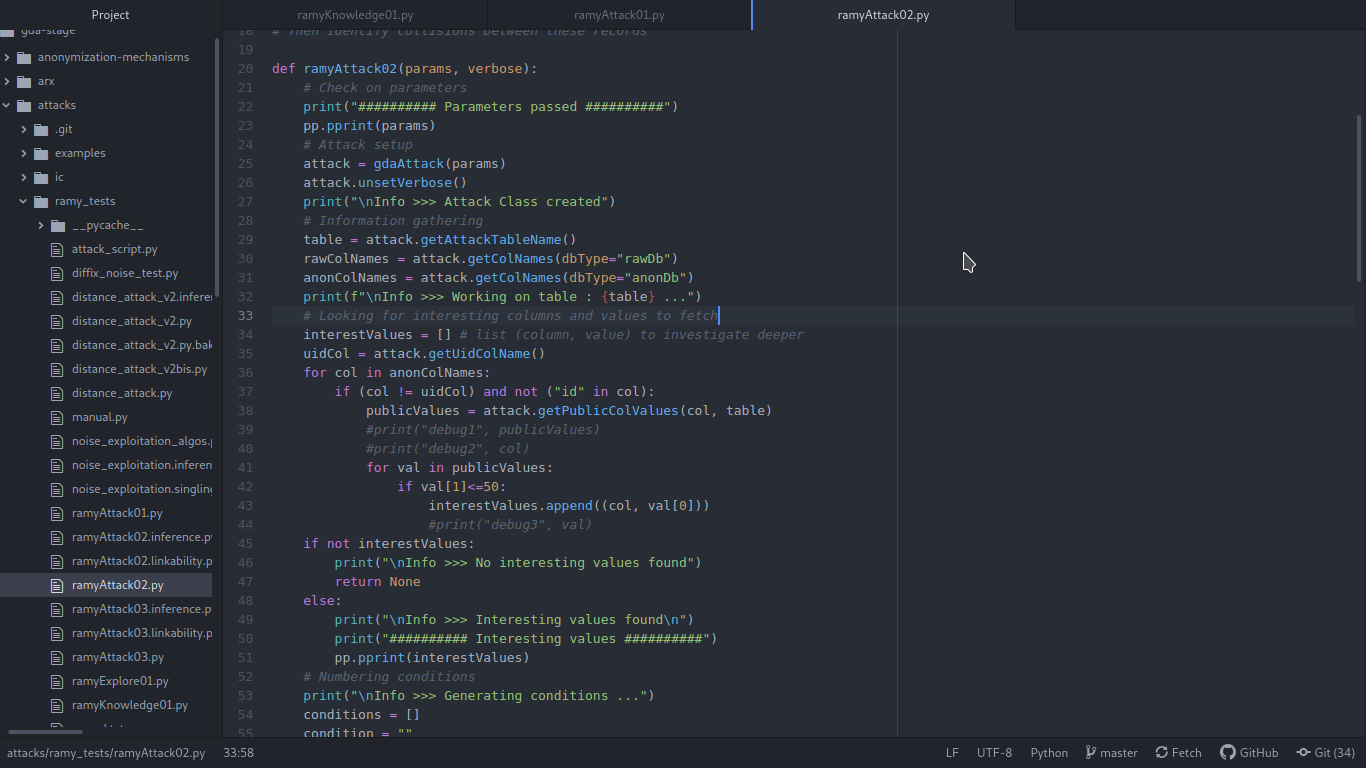
\includegraphics[width=1\linewidth]{illust01.png}
%\end{center}
%}
\end{frame}
%------------------------------------------------

\fbckg{illust05.png} % Slide background image
\begin{frame}
%\misc{ % Anything can be placed inside the \misc{} command
%Schema for the four classes
%\begin{center}
%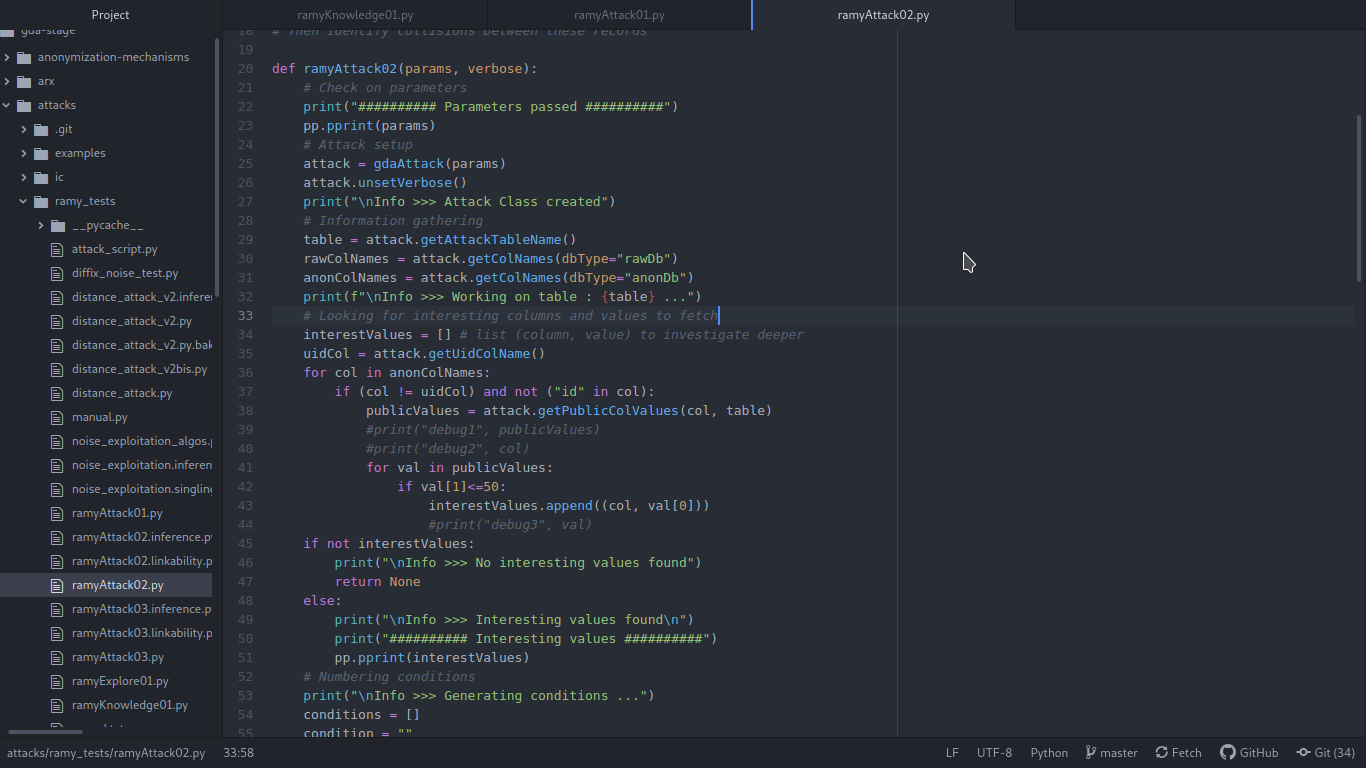
\includegraphics[width=1\linewidth]{illust01.png}
%\end{center}
%}
\end{frame}
%------------------------------------------------

\fbckg{illust06.png} % Slide background image
\begin{frame}
%\misc{ % Anything can be placed inside the \misc{} command
%Schema for the four classes
%\begin{center}
%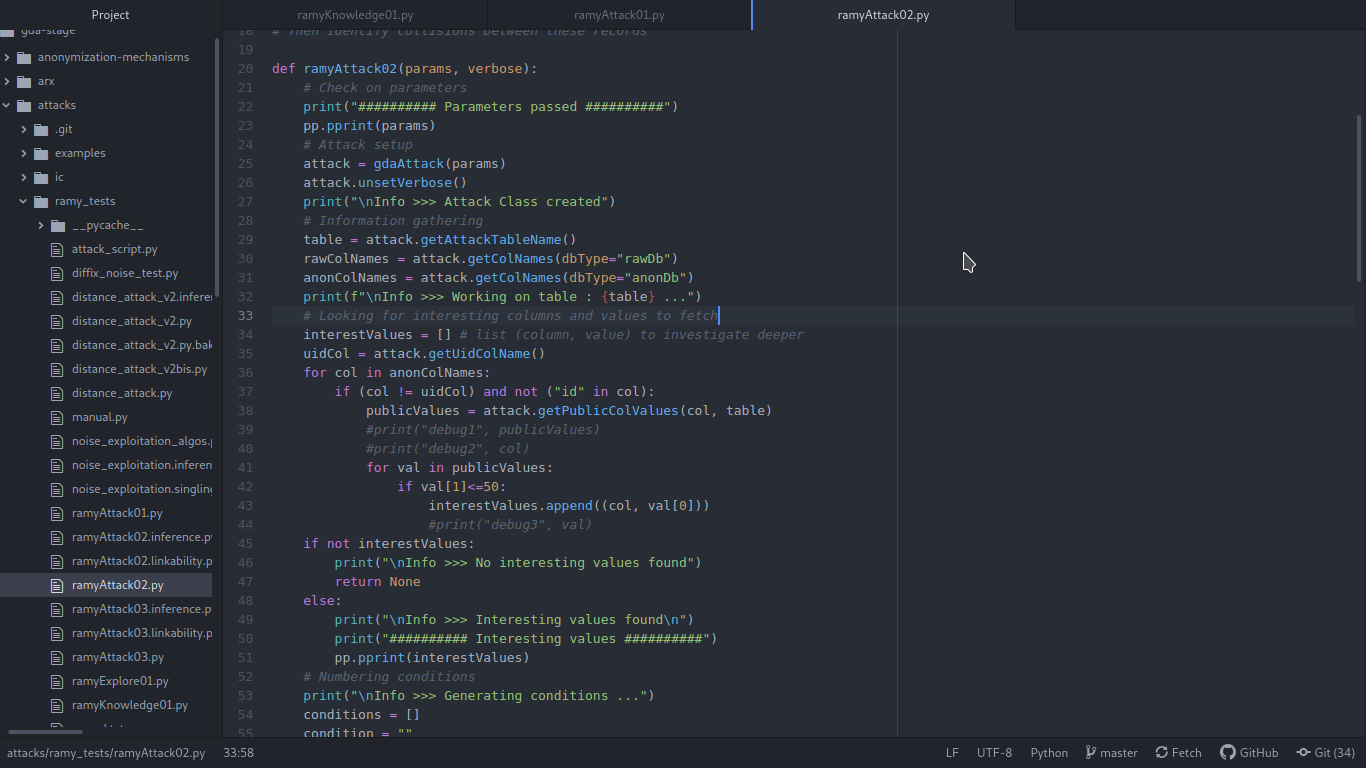
\includegraphics[width=1\linewidth]{illust01.png}
%\end{center}
%}
\end{frame}
%------------------------------------------------

\fbckg{illust07.png} % Slide background image
\begin{frame}
%\misc{ % Anything can be placed inside the \misc{} command
%Schema for the four classes
%\begin{center}
%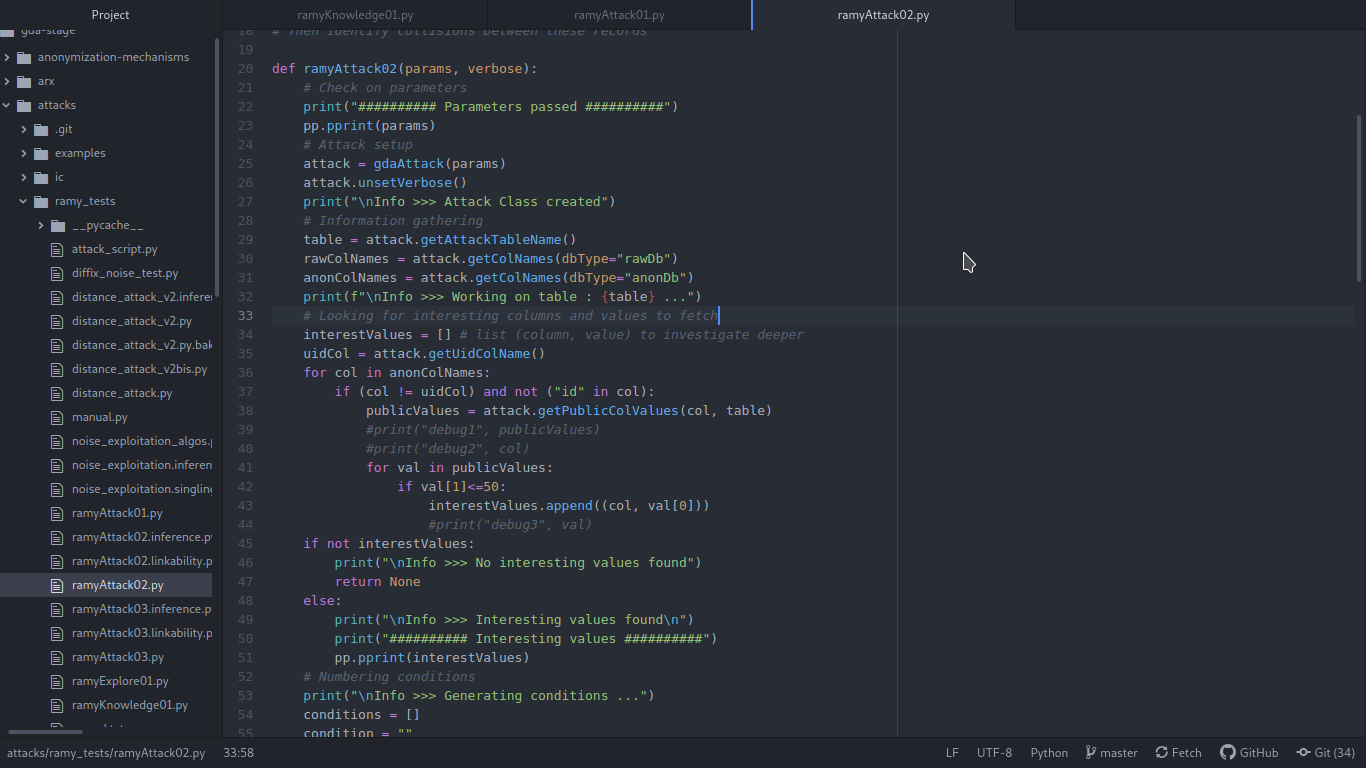
\includegraphics[width=1\linewidth]{illust01.png}
%\end{center}
%}
\end{frame}
%------------------------------------------------

\fbckg{illust08.png} % Slide background image
\begin{frame}
%\misc{ % Anything can be placed inside the \misc{} command
%Schema for the four classes
%\begin{center}
%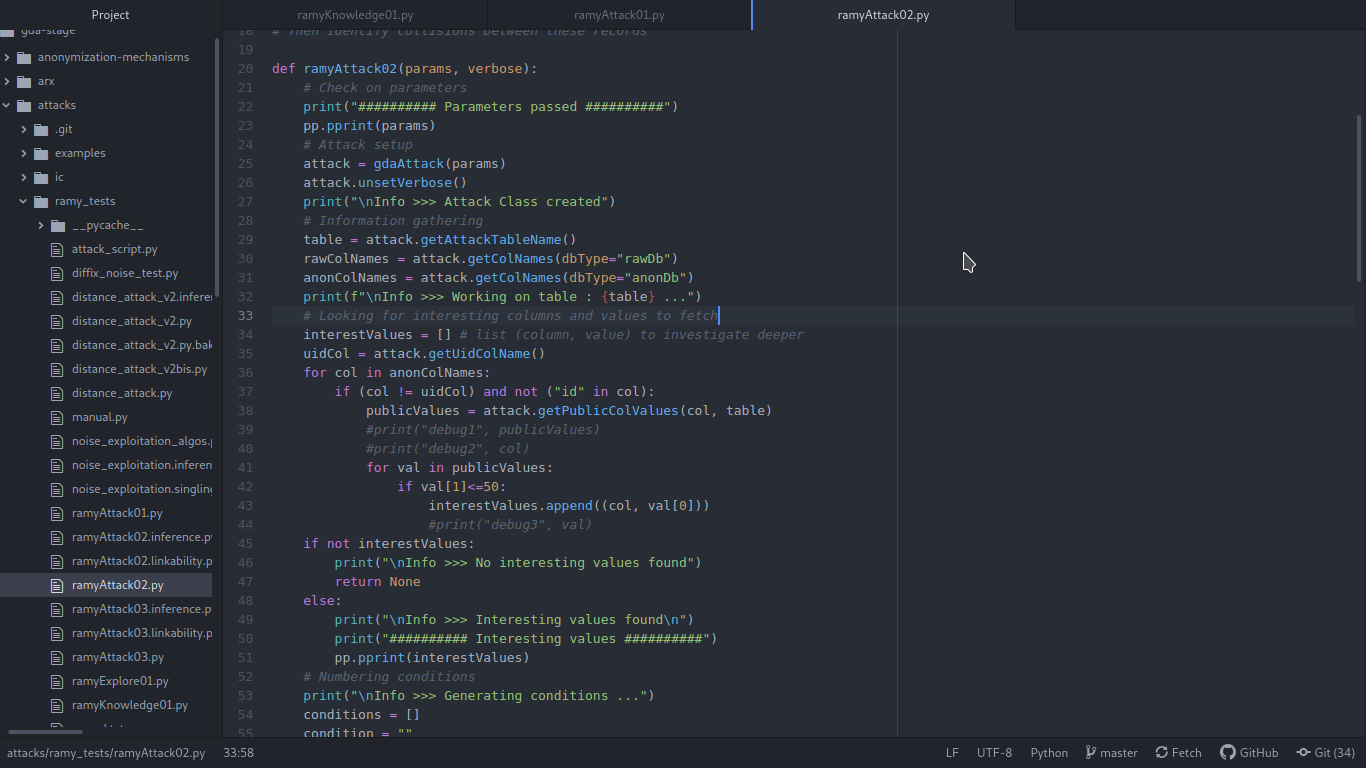
\includegraphics[width=1\linewidth]{illust01.png}
%\end{center}
%}
\end{frame}
%------------------------------------------------

\fbckg{illust09.png} % Slide background image
\begin{frame}
%\misc{ % Anything can be placed inside the \misc{} command
%Schema for the four classes
%\begin{center}
%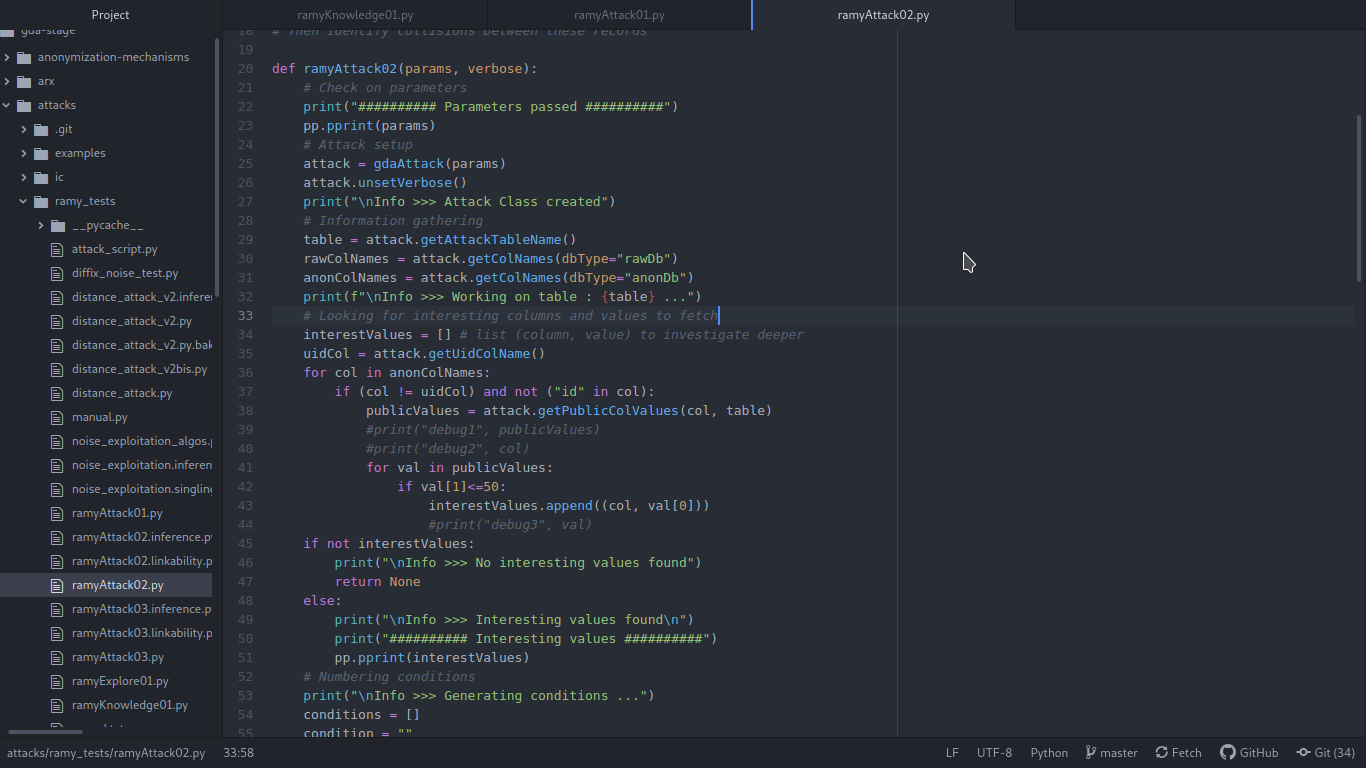
\includegraphics[width=1\linewidth]{illust01.png}
%\end{center}
%}
\end{frame}

%------------------------------------------------

\iffalse
%\fbckg{2.jpg} % Slide background image
\begin{frame}
\framedsl{explained clearly with more text} % Text in this environment will be made large, uppercase and will wrap multiple lines
\end{frame}
\fi

%------------------------------------------------

\fbckg{blank} % Slide background image
\begin{frame}
\thankyou % Inserts a thank you slide
\end{frame}

%------------------------------------------------

\iffalse
\fbckg{blank} % A blank background can be used instead of an image
\begin{frame}
\sources{ % An environment for giving credit for slide backgrounds, images will need to be scaled down if there are more than two
%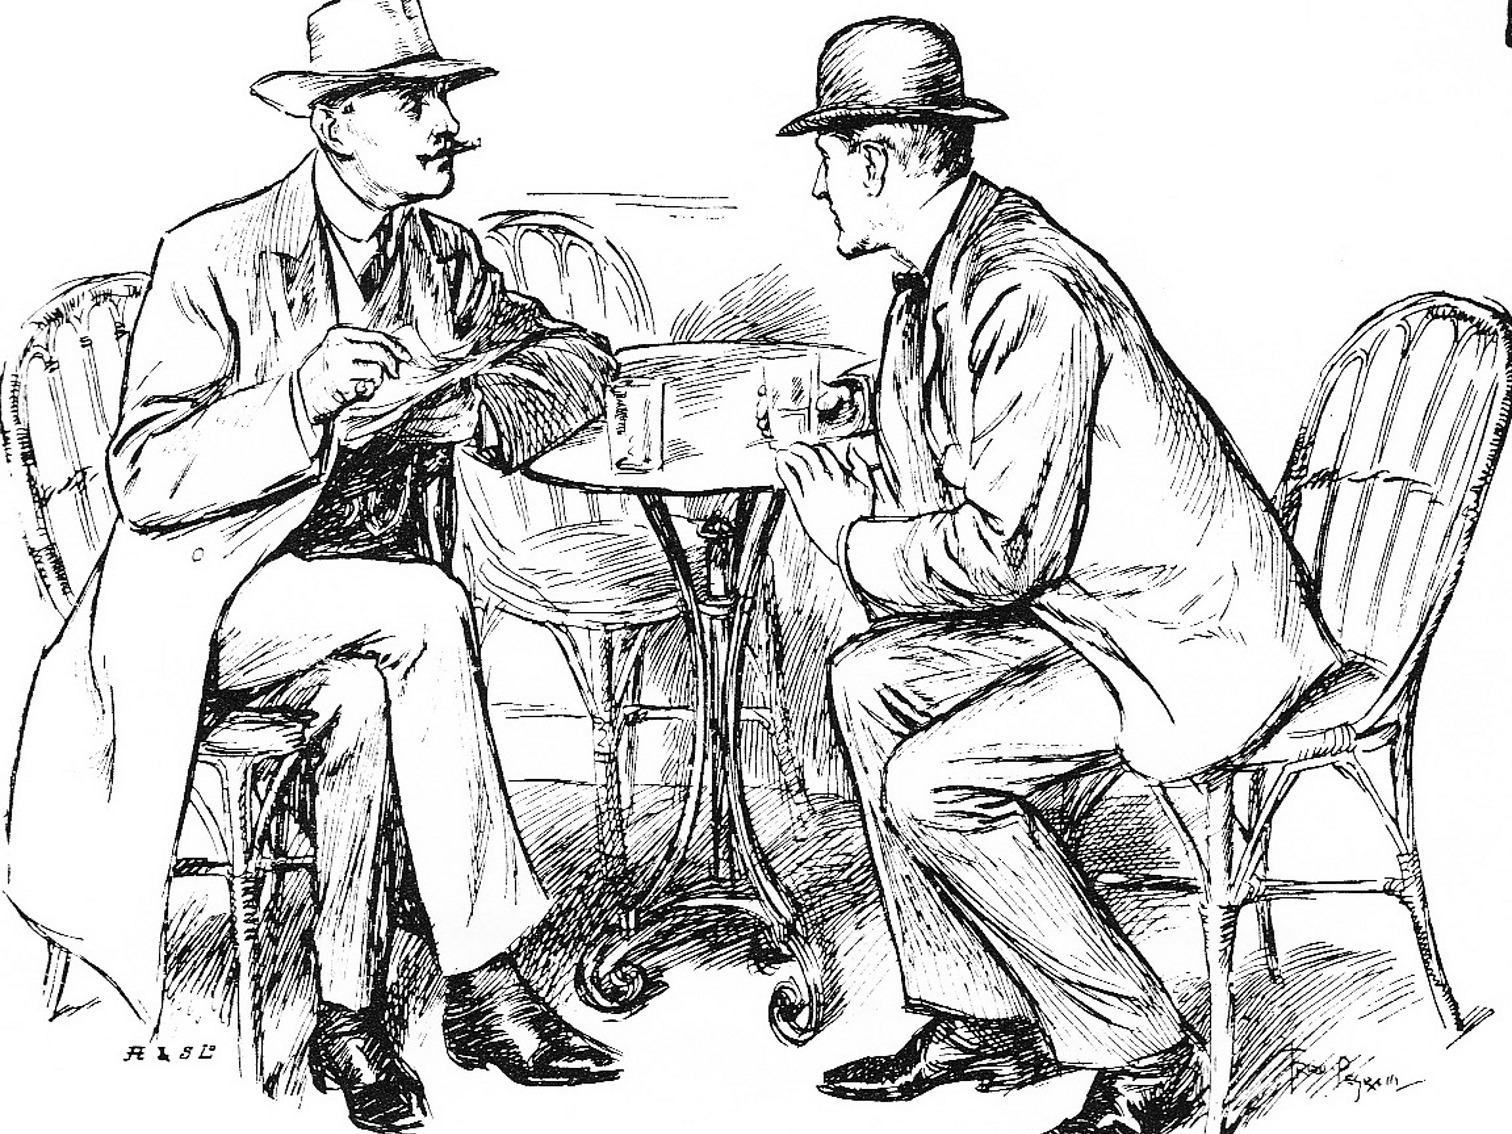
\includegraphics[scale=0.048]{1.jpg} \ flickr/lovelornpoets\\
%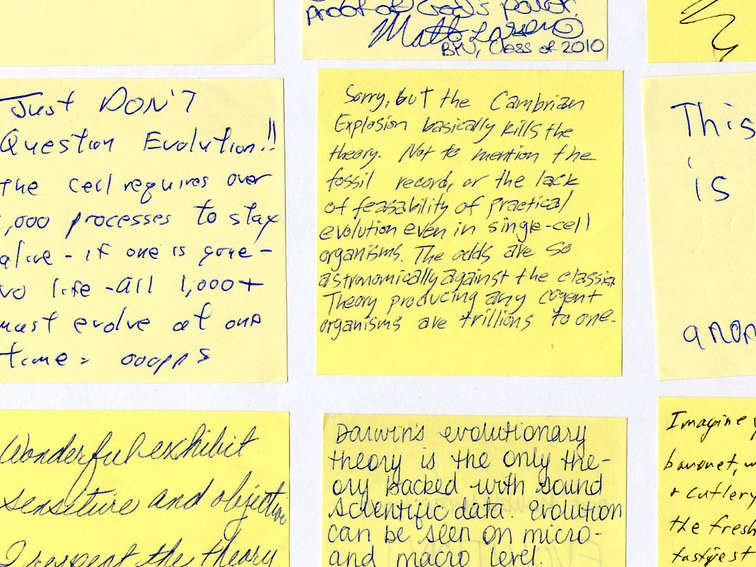
\includegraphics[scale=0.2]{2.jpg} \ flickr/apsmuseum
\bullet Benjamin Nguyen, Claude Castelluccia, Techniques d'anonymisation tabulaire : Concepts et mise en oeuvre,
Bulletin 1024, 15:23-41, 2020 \\ \\
\bullet  https://www.gda-score.org/, 28/08/2020 \\ \\
\bullet  https://pypi.org/project/gda-score-code/, 28/08/2020
}
\end{frame}
\fi

%----------------------------------------------------------------------------------------

\end{document}